\documentclass{article}
\usepackage[utf8]{inputenc}
\usepackage[T1]{fontenc}
\usepackage{geometry}
\usepackage{amsmath}
\usepackage{amsfonts}
\usepackage{hyperref}
\usepackage{graphicx}
\geometry{a4paper, total={6in,10in}}
\title{ECE 250 Project - Dota Draft Anaylsis}
\author{Mikael Huff}
\date{}
\graphicspath{ {./images/} }
\begin{document}
\maketitle


Code can be downloaded at \url{https://github.com/MikaelHuff/DotaDraftAnalysis}. Main file to be ran is mainGUI.py (recommend using the Randomize button once GUI open), that should be fine and do everything. Every file has comments explaining what the file does. Code will also be included at the end of this report. \\

The video game of Dota 2 is an online game where two teams of 5 play versus each other. Each of these 10 players will at the beginning of the game choose 1 of 123 characters to play as for that match. The game is also complex enough where this beginning of choice for heroes can be highly influential on deciding the outcome of the game. The hope of this project is to look at that initial choice by all 10 players and give some estimation on which team of 5 has an advantage before they even start to play. This project uses data that was collected thanks to the API from \url{https://www.opendota.com} which contains records of all the games played by players throughout the world. \\

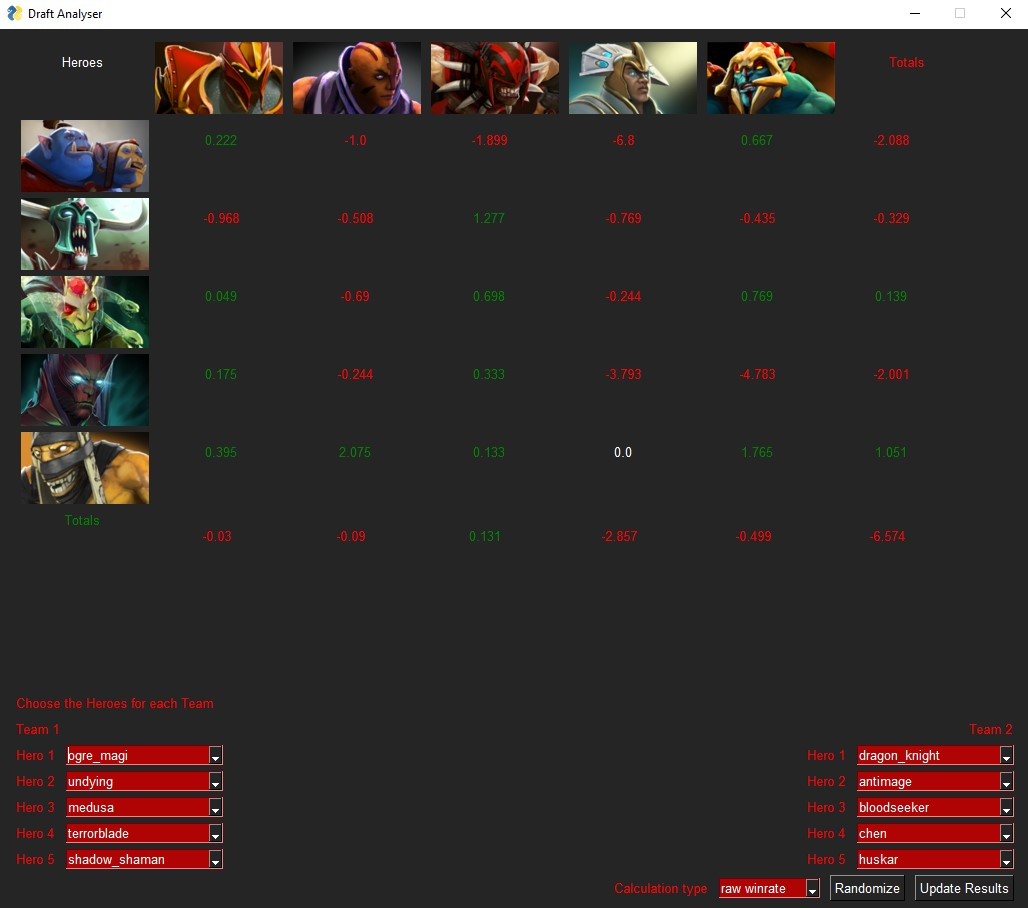
\includegraphics[width=15cm]{FullShot.jpg}

	This project has 5 python files, which I will cover briefly first to get them out of the way. dataAPI.py is the file that pulls all the necessary data from the opendota API and saves them as files. dataComp.py then takes those files and reformats the data to a more usable form. imageDownloader.py takes a folder of images (heroes) that I downloaded and chooses the required ones and moves them to a different folder called Images. mainGUI.py is the file that combines all of the other files and creates an interactable GUI for the user to use. The final file, draftAnalyser.py, in short takes a given draft of 10 heroes and returns the values to be shown at the GUI. The calculations done can be shown as 
\begin{align*}
\text{Final Score} &= \sum_{i=1}^5 K_1 \times \text{Hero rating} - \sum_{i=1}^5 K_1 \times \text{Hero rating} \\
\text{where Hero rating } &= \sum_{i=1}^5 K_2\times K_3 \times \text{matchup winrate} \\
\text{and each} K_i &= \frac{1}{1+e^{\frac{x-\mu_i}{\sigma_i}}}
\end{align*}

If each $K_i=1$, then this would be equivalent to summing up all the individual winrates (positive for team A and negative for team B) and then stating team A is better off if the value is positive. This can be done as shown \\
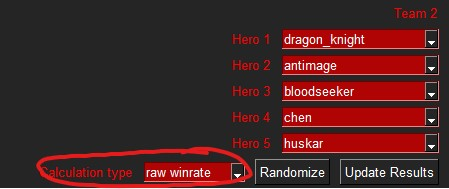
\includegraphics[width=8cm]{raw winrate}
\\

If we actually choose to use the calculation for each $K_i$, then we can see that each $K_i$ is dependent on $\mu_i$ and $\sigma_i$. This is because I assumed the data to be pulled from a normal distribution. With each x being pulled from a normal distribution, $\frac{x-\mu_i}{\sigma_i}$ is the distance from the mean in terms of standard deviations. We then pass this value into $\frac{1}{1+e^{s}}$ which is the sigmoid function. These two things together give us a function that is similar to what the CDF of the distribution would be. If a value is less than the mean, we will get a smaller number and if it is larger than the mean, we will get a larger number. The sigmoid here is important as it allows us to have a sense of direction to our distance from the mean. For each of these, we calculated our mean via the sample average and the variance via the sample variance \\

Now, to cover what each $K_i$ and its parameters cover in terms of the data being used. It is important to realize here that $K_1$ is a vector and $K_2,K_3$ are square matrices of size equal to the amount of heroes. Firstly, $K_1$ refers to the number of games a hero has been in. Consider the case where a hero X has been in $\frac{122}{5} \approx 25$ games where this hero X has played against every other hero in the game only once (ignoring twice for three heroes due to games requiring teams of 5). In this situation, every single data point regarding win rate coming from hero X is unreliable as they will all be either 1 or 0 which are extremes that are obviously not useful to consider. Then this $K_1$ in the index corresponding to hero X would have a low value that results in any information gotten from hero X's data to be practically ignored. $K_2$ which is nearly identical to $K_1$ but one step more detailed. Instead of being a heroes total games compared to the average heroes total games, we are now considering for each hero A, every other heroes games against that hero A with the mean being the average amount of games any hero has against hero A. \\

The final constant matrix $K_3$ is for win rates rather than total games. We don't in this problem consider a heroes total winrate versus the global average of 50 percent, but only a hero A's total winrate versus their winrate compared to any other hero. This $K_3$ is important, as it slightly changes the problem being solved in this project from which team will win to which team is better. This distinction refers to how the game of Dota 2 works. As this is an online game that still recieves updates from its developers, the winrates of heroes can change drastically with every update. However, the relative advantage one hero has against another hero generally barely change regardless of hero strength. For example, imagine a situation with hero A and hero B where hero A wins 75$\%$ of the games against hero B while any other hero has a 25$\%$ winrate against hero B. It is then fair to say that hero A is good against hero B. However, now imagine a change to the game occurs that causes both these percents to halve. Now, hero A's winrate against hero B would be less than 50$\%$ which would seem to mean that hero A is bad against hero B, but heroes A chance of winning would still be triple any other hero so we prefer to say hero A is good against hero B. This point means thatthe value that my program is calculating is catered more towards picking the most optimal heroes regardless of game updates, rather than winning in a single specific game version. The numbers in these examples were however, very extreme. Generally we would see winrates within the range of $[40\%,60\%]$. This is where $K_1$ and $K_2$ are very useful, because any winrate that occurs outside of this range is almost certaintly caused due to a lacking amount of data, and having 100$\%$ winrate is extremely influential, as it ought to overpower every other value in the calculation, if it were to be true but the other weights work to change this from game changing to ignored. \\

Now to cover the general usage of the program, the GUI is split into two parts, the top and the bottom. Covering the bottom side first. \\
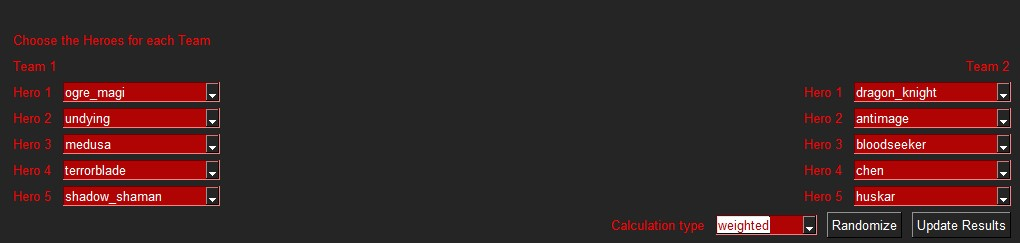
\includegraphics[width=15cm]{bottomGUI}
Here, you can see 5 drop downs on both the left and right side of the window. These correspond to each team, and each individual drop down allows for a choice amonst the 123 heroes in the game. Underneath the dropdowns, on the bottom right of the window, there is one more drop down menu and two buttons. The menu allows the user to decide if they wish to use all the constants $K_i$ defined earlier or to just use the raw winrate of each matchup. The first button "Randomize", when clicked changes the 5 drop down menus of each team to be a random selection without duplicates. The last button "Update Results", takes our 10 choices in heroes, and our calculation type and then shows the outcome in the top half of the GUI as shown \\
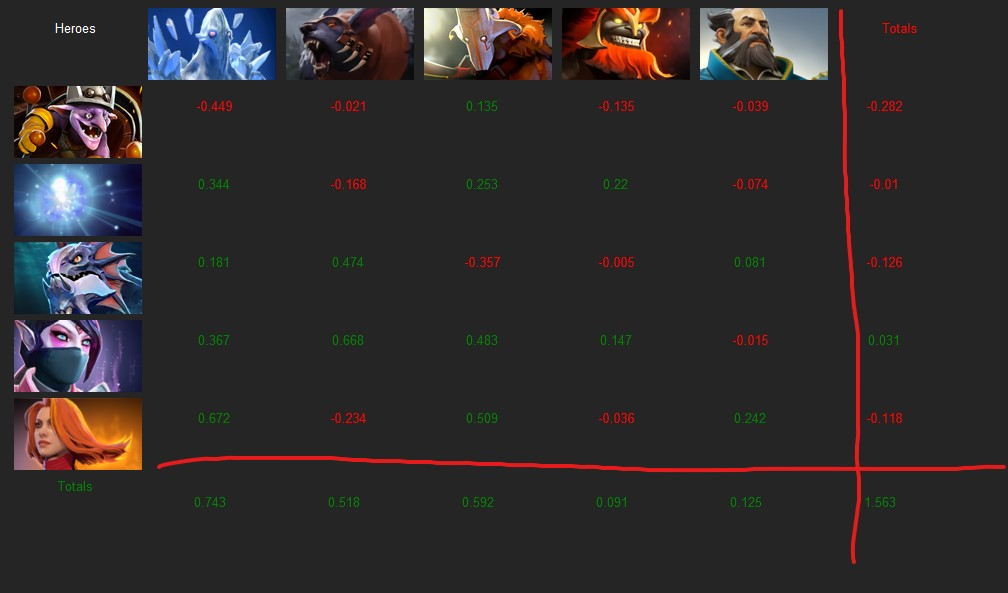
\includegraphics[width=15cm]{topGUI}
This can be split into 3 sections. For all 3, positive numbers are shown in green which mean that Team A, the team shown on the left vertically, has the advantage and the negative numbers shown in red mean that Team B, shown on top horizontally, has the advantage. The first section, being the 5 by 5 set of numbers to the top left of the red lines, shows the advantage of each matchup. These values are shown (if the option is on) with the weights from $K_2$ and $K_3$ applied. The next section is the sets of 5 numbers, either bottom left or top right of the red lines, which are the margins for each hero choice. Each of these represent how good the choice in hero is. This number has the corresponding weight from $K_1$ applied. The final value in the bottom right of the red lines, is the pure sum of the margins, which shows overall, which team is better chosen. \\

The final thing to say, is that most of the computations are done before the window even opens, meaning that choosing new heroes should be quick. And furthermore it can be updated easily with new data by just running the dataAPI.py file (Note: needs an API key to have the necessary amount of calls). The rest of the pages will include the code
\end{document}